\scanpage{322}
\deleted{$\Gamma^p(f)\circ u_p$}
\deleted{$\Gamma^p(f)$}
\[
\diagram{\begin{tikzcd}[column sep=large,row sep=large]
\Gamma^p(F_A(X))\otimes\Gamma^q(F_A(\unsure{X|Y})))\arrow[r]\arrow[d]&F_A\Gamma^p(X)\otimes F_A\Gamma^q(\unsure{X|Y})\arrow[d]\\
\Gamma^{p+q}F_A(X)\arrow[r,no head]\arrow[d]&\unsure{F_A\Gamma^{p+q}F(X)}\\
[(\Gamma^p f\circ u_p)\otimes(\Gamma^q g\circ u_q)]\circ\Delta&{}
\end{tikzcd}}
\]
\[
f,g:\diagram{\begin{tikzcd}A\arrow[r,shift left=.5ex]\arrow[r,shift right=.5ex,"{1,1}"']&X\end{tikzcd}}
\]
\[
(\Gamma^p f\circ u_p\quad\unsure{\otimes}\quad\Gamma^q g\circ u_q)
\]
\[
A\longrightarrow\Gamma^p X\qquad A\longrightarrow\Gamma^q X
\]
\[
f^{(p)}\otimes g^{(p)}
\]
\[
\diagram{\begin{tikzcd}[column sep=large,row sep=huge]
A\arrow[r,"\Delta"]\arrow[d]\arrow[drr,bend right=15,"{\text{défini par }f^{(p)}g^{(q)}\in\Gamma^{p+q}F_A(X)}"']&A\unsure{\otimes}A\arrow[r,"{(\Gamma^p f\circ u_p^{\unsure{A}})\otimes(\Gamma^qg\circ u_q)}"]&\Gamma^p(X)\otimes\Gamma^q(Y)\arrow[d]\\
{}&{}&\Gamma^{p+q}(X)
\end{tikzcd}}
\]
\margin{$f^{(p)}\otimes g^{(q)}$}
\[
\diagram{\begin{tikzcd}[column sep=huge,row sep=large]
\Gamma^p(\overbrace{F_A(X)}^{f})\otimes\Gamma^q(\overbrace{F_A(X)}^{g})\arrow[r]\arrow[d]&F_A\Gamma^p(X)\otimes F_A\Gamma^q(X)\\
\Gamma^{p+q}F_A(X)\arrow[ddr]&F_A(\Gamma^p(X)\otimes\Gamma^q(X))\arrow[u,"\unsure{\uparrow|\downarrow}"]\arrow[d]\\
{}&F_A(\Gamma^{p+q}(X))\\
{}&{}
\end{tikzcd}}
\]
\margin{$f^{(p)}\in$}
\margin{$\ni g^{(q)}$}
\margin{$\Gamma^p(f)\circ u_p\quad\otimes\quad\Gamma^q(g)\circ u_q$}
\margin{$f^{(p)}g^{(q)}$}
\inserted{$\unsure{\wedge}$}

Il suffit de prendre $X=Y=A$, $f=g=\mathrm{id}$
\[
\diagram{\begin{tikzcd}[column sep=large,row sep=huge]
A\arrow[r,"\Delta"]\arrow[drr,bend right=15,"{\text{défini par }(\mathrm{id}_A)^{(p)}(\mathrm{id}_A)^{(q)}\in\Gamma^{p+q}F_A(A)}"']&A\otimes A\arrow[r,"u_p\otimes u_q"]&\Gamma^p(A)\otimes\Gamma^q(A)\arrow[d]\\
{}&{}&\Gamma^{p+q}(A)
\end{tikzcd}}
\]
\margin{$1^{(p)}1^{(q)}=c_{pq}1^{(p+q)}$}
i.e. par $c_{pq}\mathrm{id}_A^{(p+q)}$, donc $\unsure{c_{p+q}|c_{pq}}u_{p+q}$
\figure{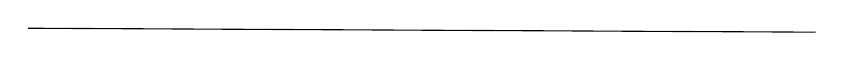
\begin{tikzpicture}\draw(0,0)--(10,-.05);\end{tikzpicture}}
\[
\diagram{\begin{tikzcd}[column sep=large]
\underbrace{\Gamma^*F(\unsure{A})}_{\otimes\text{-anneau}}\arrow[r]&\underbrace{F(\unsure{F^*|\Gamma^*}(X))}_{\otimes\text{-anneau}}
\end{tikzcd}}
\]
car $F$ commute à $\otimes$
\figure{\begin{tikzpicture}\draw(0,0)--(0,1);\end{tikzpicture}}
\margin{323}
